\documentclass[%
crop,%
tikz,%
convert={outext=.svg,command=\unexpanded{pdf2svg \infile\space\outfile}},%
multi=false%
]{standalone}%
\usepackage[utf8]{luainputenc}%
\usepackage{xspace}%
\usepackage{amsmath}%
\usepackage{amssymb}%
\usepackage{mathrsfs}%
\usepackage{mathtools}%
\usepackage{siunitx}%
\usetikzlibrary{arrows.meta,patterns,calc,backgrounds}%
\input{Definitions.tex}%
\begin{document}
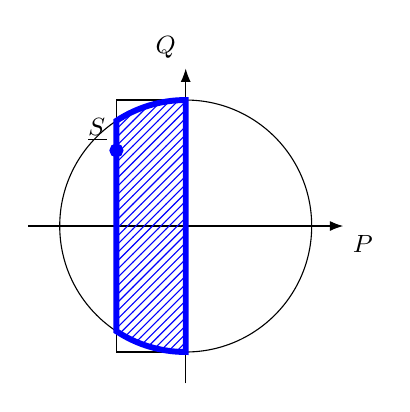
\begin{tikzpicture}[%
    show background rectangle,%
    tight background,%
    background rectangle/.style={fill=white}%
    ]
    %
% Styles
%
\tikzset{every node/.style={font=\small}};%
\tikzset{fleche/.style={->, -{Latex}}};%
\tikzset{point/.pic={\filldraw[#1] (0,0) circle[radius=0.05];}};%
\tikzset{domaine/.style={blue, line width=0.75mm}};%
\tikzset{domaine hache/.style={domaine, pattern=north east lines, pattern color=blue}};%

%
% Macros
%
\pgfmathsetmacro{\r}{1.6};%
\pgfmathsetmacro{\R}{2};%
\pgfmathsetmacro{\pthvaleur}{-0.55*\r};%
\pgfmathsetmacro{\qthvaleur}{0.6*\r};%
\pgfmathsetmacro{\angthvaleur}{acos(\pthvaleur/\r)}%
\pgfmathsetmacro{\angeuclthvaleur}{180+atan(\r/\pthvaleur)}%
\pgfmathsetmacro{\qthmaxvaleur}{\r*sin(\angthvaleur)}%

%
% Common part of the picture
%
\draw (0,0) circle[radius=\r];%
\draw[fleche] (-\R,0) -- (\R,0) node[below right] {$P$};%
\draw[fleche] (0,-\R) -- (0,\R) node[above left] {$Q$};%
\node[above left] at (\pthvaleur,\qthvaleur) {$\underline{S^{\theo}}$};%
\draw (0,-\r) -- (\pthvaleur,-\r) -- (\pthvaleur,\r) -- (0,\r);%
% Local Variables:
% mode: latex
% TeX-engine: luatex
% TeX-source-correlate-method-active: synctex
% ispell-local-dictionary: "british"
% coding: utf-8
% LaTeX-indent-level: 2
% fill-column: 120
% End:
%

    % The domain is a prtion of the circle
    \filldraw[domaine hache] (0,-\r) arc[start angle=-90, end angle=-\angthvaleur, radius=\r] --
    (\pthvaleur, \qthmaxvaleur) arc[start angle=\angthvaleur, end angle=90, radius=\r] --cycle;%

    \pic[domaine] at (\pthvaleur,\qthvaleur) {point};%
\end{tikzpicture}
\end{document}
% Local Variables:
% mode: latex
% TeX-engine: luatex
% TeX-source-correlate-method-active: synctex
% ispell-local-dictionary: "british"
% coding: utf-8
% LaTeX-indent-level: 4
% fill-column: 100
% End:
